%Januar 2021 - März 2021


\documentclass[12pt]{article}

\usepackage{multicol}
\usepackage{geometry}
\usepackage{blindtext}
\usepackage{setspace}
\usepackage{hyperref}
\usepackage[headsepline=0.8pt, footsepline =0.8pt]{scrlayer-scrpage}
\usepackage{listings}
\usepackage{subcaption}
\usepackage{tabularx}
\usepackage{xurl} %Formats \url{}-entrys better
\usepackage{color, colortbl}
%\usepackage{pdfpages}
\usepackage{amssymb}
\usepackage{caption}
\usepackage{subcaption}
\usepackage{float}


\geometry{a4paper, top=25mm, left=35mm, right=25mm, bottom=25mm, headsep=13mm, footskip=12mm, head=14.5pt}

%encoding
%--------------------------------------
\usepackage[utf8]{inputenc}
\usepackage[T1]{fontenc}
%--------------------------------------

%German-specific commands
%--------------------------------------
\usepackage[ngerman]{babel}
%--------------------------------------

%Hyphenation rules
%--------------------------------------
\usepackage{hyphenat}
%--------------------------------------


\usepackage{graphicx}
\graphicspath{ bilder/}

\hypersetup{pdfborder={0 0 0}}


\newcommand{\Autor}{Andreas Schmider}

\newcommand{\Bearbeitungszeitraum}{2 Semester}
\newcommand{\Kurs}{TINF19B3}


% Images
\newcommand{\DHBWLogoDeckblatt}{
\includegraphics[width=4.5cm]{Logos/dhbw-logo}}
\newcommand{\KernPackages}{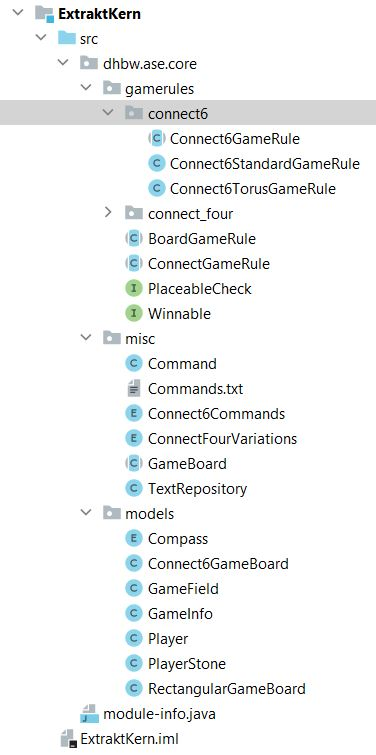
\includegraphics[height=12cm]{Bilder/KernModul_Packages}}
\newcommand{\PluginPackages}{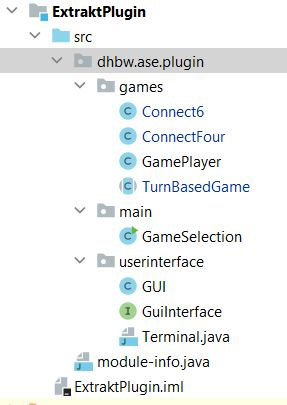
\includegraphics[height=7cm]{Bilder/PluginModul_Packages}}
\newcommand{\BridgePattern}{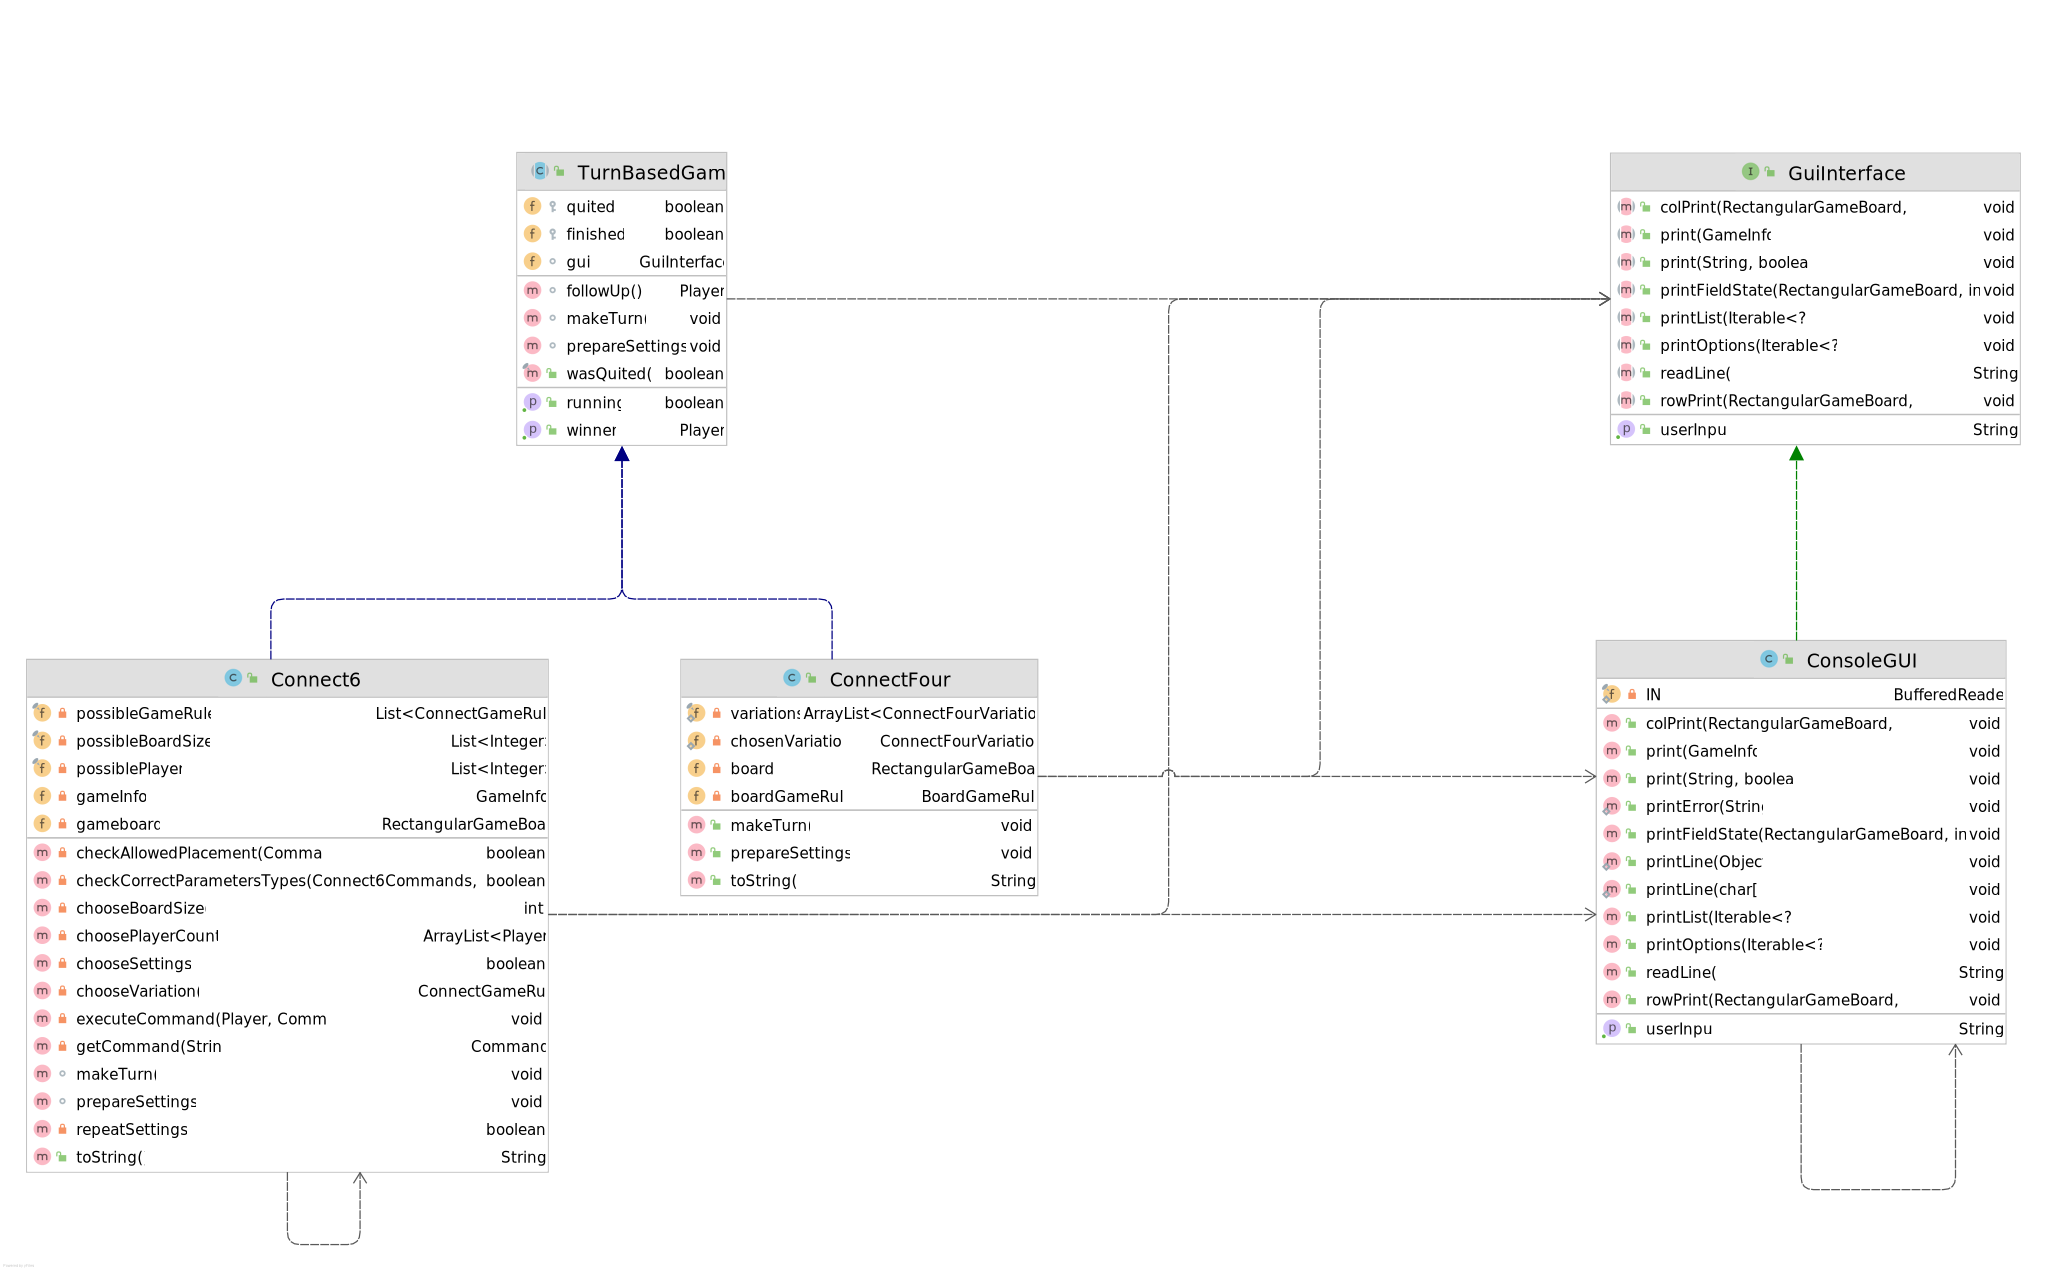
\includegraphics[height=7cm]{Bilder/Bridge_complete}}
\newcommand{\PrintList}{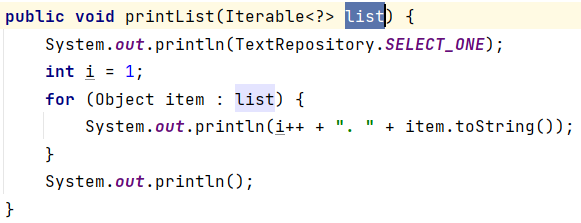
\includegraphics[width=15cm]{Bilder/printList}}
\newcommand{\RowPrint}{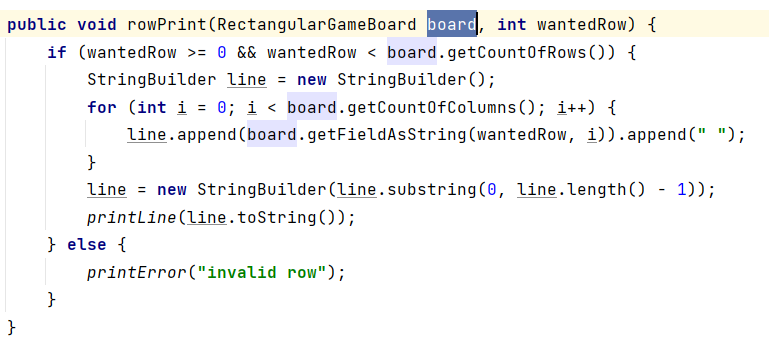
\includegraphics[width=15cm]{Bilder/rowPrint}}
\newcommand{\pkgGamerule}{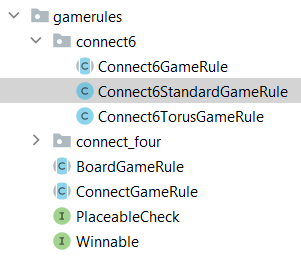
\includegraphics[width=7cm]{Bilder/gamerules}}
\newcommand{\boardGR}{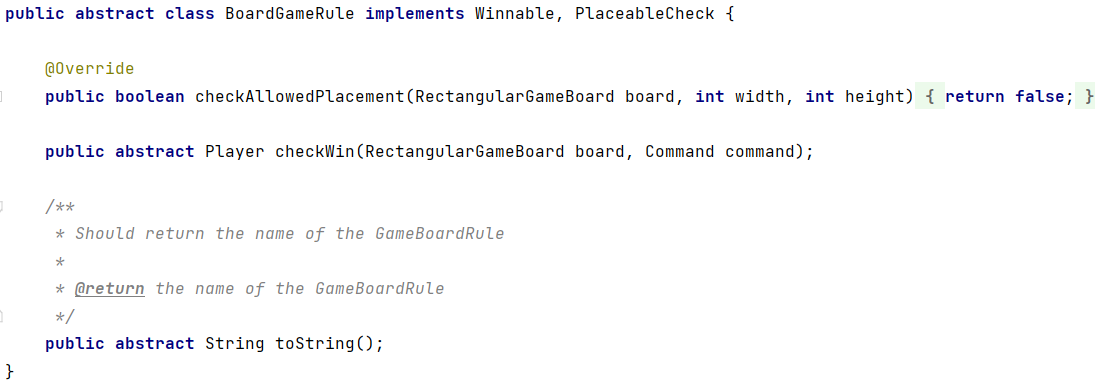
\includegraphics[width=15cm]{Bilder/BoardGameRule}}
\newcommand{\torus}{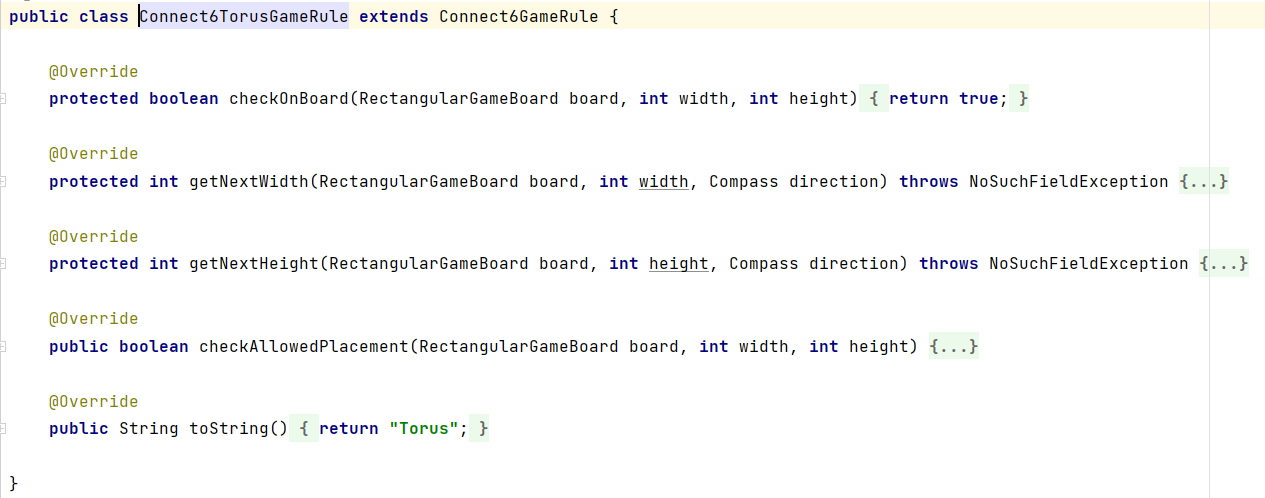
\includegraphics[width=15cm]{Bilder/Torus}}

\newcommand{\Titel}{Kleine Spielesammlung von 4-Gewinnt Versionen}
\newcommand{\Abschluss}{Bachelor of Science}
\newcommand{\Studiengang}{Studiengang Informationstechnik}

\newcommand{\Ort}{Karlsruhe}

%\newcommand{\Abgabedatum}{16.02.2021}


\begin{document}
\onehalfspacing
\pagenumbering{Roman}
	\begin{titlepage}
		{\DHBWLogoDeckblatt}\\[2cm]
		\begin{center}
			\vspace*{-2cm}
			{\Huge \Titel}\\[2cm]
			{\Large \Abschluss}\\[0.5cm]
			{\large \Studiengang}\\[0.5cm]
			{\large an der}\\[0.5cm]
			{\large Dualen Hochschule Baden-Württemberg Karlsruhe}\\[0.5cm]
			{\large von}\\[0.5cm]
			{\large\bfseries \Autor}\\[1cm]
			{\large Abgabedatum 30. April 2022}
			\vfill
		\end{center}
		\begin{tabular}{l@{\hspace{1cm}}l}
			Bearbeitungszeitraum & \Bearbeitungszeitraum \\
			Kurs & \Kurs \\
		\end{tabular}
	\end{titlepage}

\newpage

\newpage

\thispagestyle{empty}
\setcounter{tocdepth}{2}
\tableofcontents

\newpage

%\thispagestyle{empty}
\thispagestyle{plain}
\cleardoublepage
\addcontentsline{toc}{section}{\listfigurename}
\listoffigures

\addcontentsline{toc}{section}{\listtablename}
\listoftables

\newpage


\thispagestyle{plain}
\pagenumbering{arabic}

\section{Beschreibung der Software}

\textbf{Beschreibung der Funktionalität}
\\
\noindent Aus einem alten Projekt existiert schon ein Connect6 Spiel, das in der Konsole gespielt wird. Dabei
gibt es einige Einstellungen die während des Programms noch gesetzt werden können. Somit kann
es von zwei bis vier Spielern gespielt oder die Spielfeldgröße auf 18x18 oder 20x20
festgelegt werden. Eine der größeren Auswirkung hat die Auswahl der Spielregeln.
Connect6 ist ähnlich wie Vier gewinnt und Ziel ist es mehrere Steine in eine Reihe zu legen.
Connect6 wird dabei aber auf einem Brett gespielt, das eben auf dem Boden liegt. So fallen die
Steine nicht bis in die letzte Zeile sondern bleiben an ihrem Platz. Ebenso werden pro Zug zwei
Steine pro Spieler gesetzt.
Bei der Standart-Spielregel zählen die Steine nur bis zum Spielfeldrand. Es gibt aber auch die
Torus-Version, bei dem die Steinreihen über den Rand hinaus gezählt werden. So beginnt das
Spielfeld erneut von oben, wenn man aus der untersten Zeile eins nach unten gehen würde.
\\

Zusätzlich soll in Zukunft auch noch Vier Gewinnt mit unterschiedlichen Variationen/Regeln implementiert werden. Bisher wurden nur die Grundsteine dafür gelegt. Bei dieser Spielesammlung soll es möglich sein mit wenig Aufwand neue Spielregeln/Variationen oder sogar ganz neue Spiele (die einen ähnlichen Aufbau haben) zu implementieren.
\\

Bei der Entwicklung dieser Software wurde zwar darauf geachtet einen möglichst strukturierten und einfachen Code zu erstellen,
es wurde sich aber nicht direkt an die in dieser Vorlesung besprochenen Themen gehalten. Es wurde zwar versucht die DRY-Regel anzuwenden, 
da diese mir schon selber in den Sinn gekommen ist, aber wie ich später festgestellt habe wurde diese nicht überall umgesetzt. Ebenso habe ich öfters kleinere Code Reviews vorgenommen und refactored, da mir immer wieder beim erneuten Anschauen aufgefallen ist, wie unverständlich der Code ist. Da der Code ursprünglich von einer Programmieraufgabe am KIT stammt, mussten auch Kommentare verwendet werden. Nachdem ich diesen Code aber nach über 3 Jahren wieder angeschaut habe ist mir klar geworden, dass trotz vieler Kommentare der Code sehr schwierig zu lesen ist.
\\ 

\noindent  \textbf{Beschreibung des Kundennutzens}
Der Kunde erhält Spaß und Unterhaltung.
\\

\noindent \textbf{Verwendete Technologien}
- Java
- JUnit 5
- IntelliJ
\\

\noindent \textbf{Link zum Repository}
\url{https://github.com/a-schmider/ASE_Substrat}





\newpage
\section{Unit tests}
Mit den bisher erstellten Tests werden ?\% der Programmzeilen abgedeckt. Dies wurde mittels Code Coverage ermittelt. IntelliJ bietet dies standardmäßig schon an und zeigt genau welcher Code ausgeführt wurde und welcher nicht. ?\% ist sehr wenig aber auch nicht verwunderlich bei diesen kleinen und wenigen Tests. 

\begin{figure}[H]
\centering
{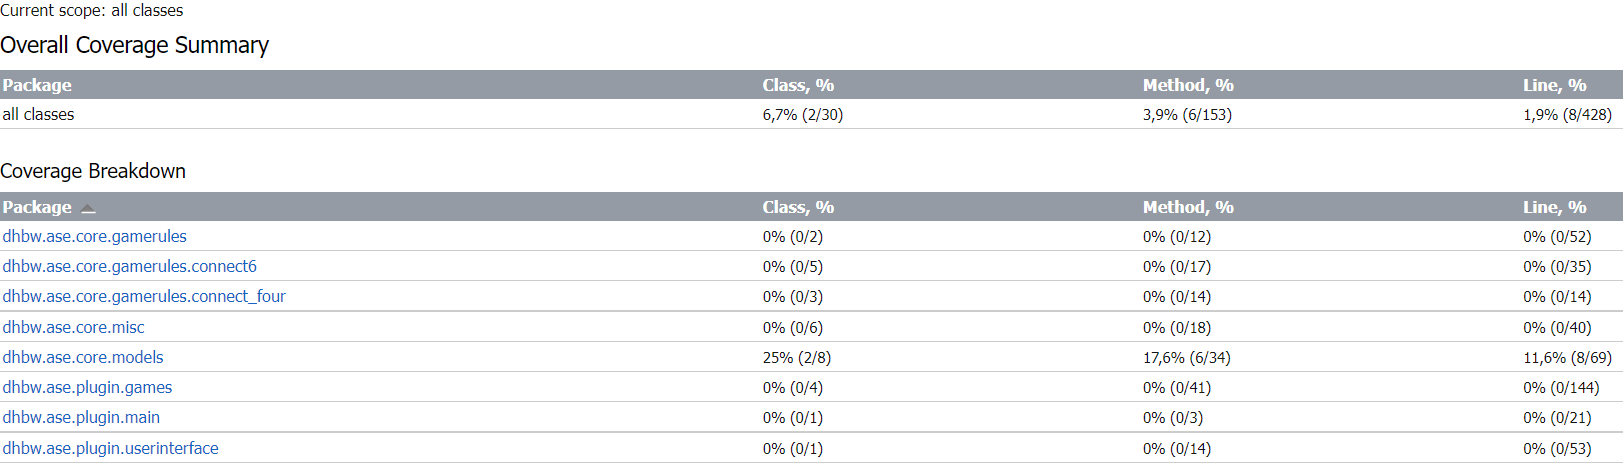
\includegraphics[width=13cm]{Bilder/CoverageAll}}
\caption{Test-Coverage über das komplette Programm}
\label{fig:CoverageAll}
\end{figure}


Wenn man sich aber die die getesteten Klassen ansieht, sieht das schon ganz anders aus. Dort wurde 100\% der Zeilen abgedeckt.

\begin{figure}[H]
\centering
{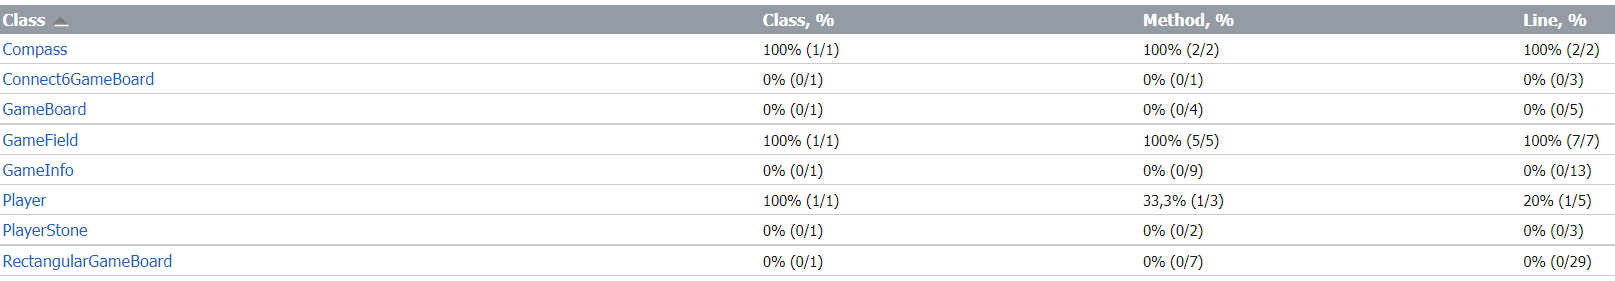
\includegraphics[width=13cm]{Bilder/CoverageModel}}
\caption{Test-Coverage für die getesteten Klassen}
\label{fig:CoverageModel}
\end{figure}


\subsection{ATRIP}

\subsubsection{Automatic}
Damit die Test automatisch ausgeführt werden, wurde in IntelliJ ein Run Configuration erstellt, womit alle Tests ausgeführt werden. Damit sich nach einer Änderung keine Fehler einschleichen, wurde auch in der Normalen Run Konfiguration für das Programm festgelegt, dass die Test im vor hinein ausgeführt werden sollen, bevor das Programm gestartet wird. 

\begin{figure}[H]
\centering
{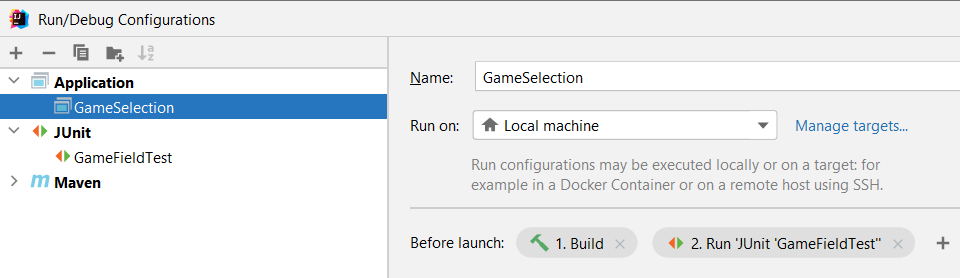
\includegraphics[width=8cm]{Bilder/AutomatedTests}}
\caption{Run-Konfiguration des Programmes}
\label{fig:AutomatedTests}
\end{figure}

Sofern die Projekt-Dateien auch im Git-Repository hinterlegt sind, haben alle Entwickler diese Konfigurationen zur Verfügung und können diese Verwenden.


\begin{figure}[H]
\centering
{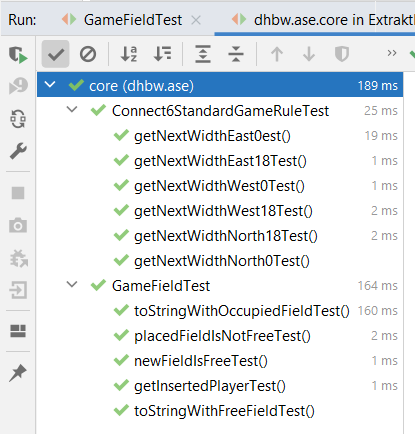
\includegraphics[width=13cm]{Bilder/TestResults}}
\caption{Automatisierung der Tests}
\label{fig:TestResults}
\end{figure}


\newpage

\subsubsection{Thorough}
Vieles in meinem Programm arbeitet mit anderen Klassen zusammen. So ist es nicht so einfach möglich mit Unit Tests zu testen, ob die Spielereingaben korrekt sind. Dies würde sich über mehrere Berichte ziehen und es würde ein Integrationstest werden. 

Ein grundlegende Funktion, worauf vieles aufbaut, sind die GameFields. Also die einzelnen Felder auf die ein Stein gesetzt werden kann. Deshalb wurden diese als erstes getestet.


\subsubsection{Repeatable}
Bei den getestet Klassen wurde darauf geachtet, dass die Tests nicht von zufälligen Eingaben oder ähnlichem abhängig sind. Somit sollten die Test beliebig wiederholt werden können und immer das Gleiche Ergebnis liefern.

\subsubsection{Independent}
Alle Tests wurden so aufgebaut, das alles, was für die Tests benötigt wurde auch nur in diesem einen Test erstellt wird. So können die Tests in beliebiger Reihenfolge ausgeführt werden.

\subsubsection{Professional}
Damit die Tests einfach zu verstehen sind, wurden die AAA Regeln bei allen Tests angewandt. Jedoch waren bei einigen Tests nicht alle Schritte notwendig und wurden deshalb weggelassen . Zu sehen ist das zum Beispiel bei dem Test mit Mocks in Abbildung \pageref{fig:Mock}.

\newpage

\subsection{Mocking}
Um die Klasse GameField zu testen wurden Mocks verwendet. Genauer gesagt, bei der toString-Methode. Diese Methode gibt den Wert, von dem Spielstein als Text zurück, der auf diesem Feld liegt. Dafür wird natürlich eine Instanz der Klasse Spieler verwendet. Dementsprechend wird dieses Objekt gemocked. Eigentlich will die GameField-Klasse aber den Spielstein, der auch noch in dem Spieler liegt. Deshalb wird der Spielstein auch gemocked. Die Player-Instanz verwendet dann die gemockte PlayerStone-Klasse. Schluss endlich kann das GameField getestet werden ohne die anderen Klassen zu verwenden.


\begin{figure}[H]
\centering
{\includegraphics[width=13cm]{Bilder/Mock}}
\caption{Verwendung von Mocks bei Unit-Tests}
\label{fig:Mock}
\end{figure}




\newpage
\section{Programming Principles}



\subsection{SOLID}


\subsubsection{Single-Responsibility-Principle}
Im Code wurde das bei den Spielregeln angewendet. Für jede Spielversion gibt es eine Klasse die nur überprüft, ob ein Zug gemacht werden darf und ob ein Gewinner vorliegt. So gibt es bisher zwei Spielvarianten für Connect6 die in unterschiedlichen Klassen implementiert sind und nicht auf eine Helper-Klasse o.ä. angewiesen sind und dort die Spielvariante abfragen müssen, um zu entscheiden, ob ein Zug erlaubt ist oder nicht. Definiert wurde das über Interfaces und der abstrakten BoardGameRule-Klasse. Die davon abgeleiteten Klassen implementieren dafür weitere Methoden, die das besser strukturieren, aber keine, die zusätzliche , ungewollte Funktionen implementieren.

\begin{figure}[H]
\centering
{\boardGR}
\caption{Die abstrakte BoardGameRule-Klasse}
\label{fig:boardGR}
\end{figure}



\subsubsection{Open/Closed-Principle}
Angewendet wurde das auf die Spielregeln. Zu Beginn gab es nur zwei Klassen für Spielregeln, die BoardGameRule- und die ConnectGameRule-Klassen. In ConnectGameRule wurde der grundsätzliche Ablauf für diese Art von Spielregeln erstellt. Durch die Unterklassen können aber neue Varianten implementiert werden, im Code mit den Connect6StandardGameRule- und Connect6TorusGameRule-Klassen. So könnten in Zukunft noch viele weitere Spielregel erstellt werden, welche diese Regeln anpassen ohne bestehenden Code zu ändern.

\begin{figure}[H]
\centering
{\torus}
\caption{Die Connect6TorusGameRule-Klasse}
\label{fig:torus}
\end{figure}



\subsubsection{Liskov-Substitution-Principle}
Dieses Prinzip wurde bei den Spielbrettern verletzt. Es wurde nämlich ein quadratisches Spielfeld als Unterklasse eines Rechteckigen Spielfelds implementiert. Somit verhält sich das quadratische Spielfeld aber nicht nicht mehr wie ein Rechteckiges Spielfeld und schränkt die Funktionalität sogar ein, anstatt sie zu erweitern.
Es gibt zwar keine Methoden um die Länge und Breite zu setzen aber einen Konstruktor, der diese setzt. Dort könnte zwar ein Fehler geworfen werden aber das führt wieder zu \glqq schlechtem \grqq Code. Deshalb sollte dort ein neues Konstrukt angestrebt werden.



\subsubsection{Interface-Segregation-Principle}
Bisher gibt es in diesem Projekt nur drei Interfaces. Eins für die GUI und zwei für Spielregeln. Bei den Interfaces für Spielregeln gibt es das Winnable Interface, das die Methode checkWin(...) und das PlaceableCheck Interface, das eine checkAllowedPlacement(...) definiert. Bisher werden diese Zwei nur von der Klasse BoardGameRule verwendet. In Zukunft könnte es aber ein Spiel geben, z.B. Monopoly, bei dem es zwar einen Gewinner gibt, aber jeder Zug erlaubt ist sodass nur Winnable und nicht PlaceableCheck implementiert werden müsste.



\subsubsection{Dependency-Inversion-Principle}
Normalerweise wird Dependency-Inversion verwendet um die Abhängigkeiten innerhalb des Programms umzudrehen. In diesem Programm wurden nur zwei Schichten der Clean-Architecture erstellt. Diese wurden auch erst sehr spät implementiert. Deshalb wurde nur versucht die Abhängigkeiten zwischen den Schichten zu regeln, damit nur die Äußeren Schichten von den Inneren Schichten abhängig sind. Dafür waren aber alle Abhängigkeiten schon in die richtige Richtung.
Der erste Schritt zur Dependency-Inversion ist die Dependency Injection. Zumindest diese wurde an einigen Stellen umgesetzt. Zum Beispiel bei der Connect6-Klasse aus der Plugin-Schicht und der ConnectGameRule-Klasse aus dem Kern verwendet. Die Connect6-Klasse besitzt drei Listen. Eine für die möglichen Spielregeln, eine für die möglichen Spielbrettgrößen und eine für mögliche Anzahl an Spielern. Alle drei Listen werden über den Konstruktor übergeben. Somit wird an dieser Stelle Dependency Injection angewandt.


\begin{figure}[H]
\centering
{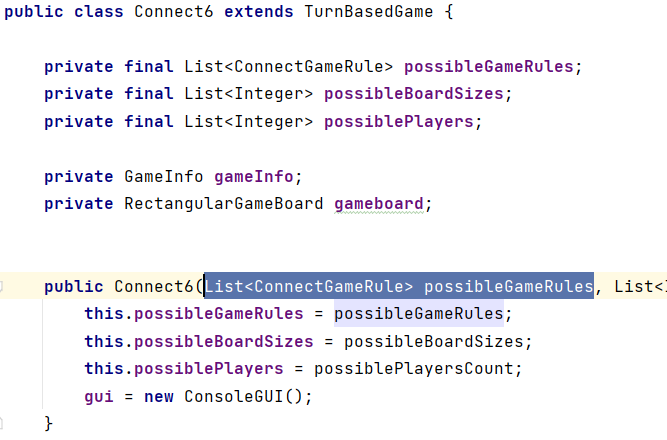
\includegraphics[width=13cm]{Bilder/DependencyInjection}}
\caption{Die Dependency Injection bei der Connect6-Klasse}
\label{fig:DependencyInjection}
\end{figure}



\subsection{GRASP}
Im laufe der Vorlesung wurden neun Faktoren von General Responsibility Assignment Software Patterns/Principles (GRASP) besprochen. Davon wurden aber nur zwei (Low Coupling und High Cohesion) genauer besprochen und deshalb sollen in diesem Dokument auch nur diese beiden thematisiert werden.



\subsubsection{Low Coupling}
Ein gutes Beispiel dafür ist das GuiInterface. Dieses besitzt eine Methode printList(Iterable<?>). Für diese Methode wird nur vorausgesetzt, dass eine Element übergeben werden muss über das iteriert werden kann. Es wäre auch möglich eine List<?> anstatt des Iterable<?> zu nehmen, da eine Liste auch das Iterable Interface implementiert und das in der Methode genutzt wird. Wenn aber eine Liste verwendet wird schränkt man die verwendbaren Klassen ein, obwohl das gar nicht nötig wäre.
\\

\begin{figure}[H]
\centering
{\PrintList}
\caption{Die printList-Methoden Implementierung}
\label{fig:printList}
\end{figure}


Das GuiInterfaces enthält ebenfalls eine rowPrint(RectangularGameBoard)-Methode. RectangularGameBoard ist diesmal aber kein Interface sondern eine normale Klasse. Indem davon Unterklassen erstellt werden, wie Connect6GameBoard, können auch diese für Low Coupling verwendet werden. 
\\

\begin{figure}[H]
\centering
{\RowPrint}
\caption{Die rowPrint-Methoden Implementierung}
\label{fig:rowPrint}
\end{figure}

Die rowPrint Methode verwendet folgende drei Methoden der übergebende Klassen.
\begin{itemize}
\item getCountOfRows
\item getCountOfColumns
\item getFieldAsString
\end{itemize}

Es wäre auch möglich ein Interface zu erstellen, dass diese drei Methoden unterstützt. So wäre es nicht notwendig, dass das übergebende Objekt eine Unterklasse oder selber vom Typ RectangularGameBoard ist. Zum Beispiel könnten dann auch Tabellen unterstützt werden, die gar nichts mit Spielbrettern zu tun haben. Dies ist für diese Spielesammmlung aber nicht interessant, da nur Spielbretter verwendet werden. Somit könnte aber noch mehr Unabhängigkeit erzielt werden.



\newpage
\subsubsection{High Cohesion}
Um eine hohe Kohäsion zu erhalten, sollte versucht werden, Klassen oder Programmteile die zusammen arbeiten auch möglichst nahe beieinander zu halten z.B. in Packages oder Modulen. Ebenso sollte jede Klasse nur für eine Aufgabe zuständig sein (s. Single-Responsibility-Principle). Damit lässt sich schneller erkennen in welchem Bereich Änderungen vorgenommen werden müssen und welche andere Klassen davon betroffen sein könnten. Zu Kohäsion zählt aber auch wie gut die Daten und die Methoden einer Klasse zusammen passen und arbeiten.

Um eine hohe Kohäsion zu erreichen werden in diesem Projekt hauptsächlich Packages verwendet. Das Package (gamerules), dass für die Spielregeln verantwortlich ist, zeigt dies ganz gut. In diesem Package liegen die abstrakten Klassen und die Interfaces welche diese implementieren. Darin gibt es weitere Packages für die genauen Spielregeln der einzelnen Spiele (connect6 und connect\_four). Sobald etwas an einem Interface oder der abstrakten Klassen geändert wird, kann erkannt werden, dass alle anderen Klassen in diesem Package davon betroffen sein könnten.

\begin{figure}[H]
\centering
{\pkgGamerule}
\caption{Das gamerule-Package}
\label{fig:pkgGamerule}
\end{figure}



\subsection{DRY}
DRY steht für \glqq Don't repeat yourself \grqq. So soll möglichst kein Code mehrfach vorhanden sein und damit verhindern, dass der Quellcode unnötig groß und es möglicherweise zwei unterschiedliche Verfahren für die gleiche Sache verwendet wird. Natürlich können grundlegende Befehle nicht nur einmal verwendet werden aber es sollte darauf geachtet werden, das falls zwei Abschnitte eine ähnliche Funktion implementieren und nur minimale Unterschiede aufweisen, diese so anzupassen, dass die Unterschiede durch Parameter oder Verzweigungen generiert werden. Somit muss nur an genau einer Stelle etwas geändert werden und alle Funktionen die darauf aufbauen erhalten diese Änderung und müssen nicht manuell angepasst werden.



\newpage
\section{Clean Architecture}
Dieses Programm wurde in zwei Schichten aufgeteilt. Dem Kern-Modul, in dem die ganzen Strukturen liegen, und dem Plugin-Modul, in dem momentan die Ausgabe/GUI realisiert wird. Um sicherzustellen, dass die Klassen im Kern die Plugins nicht kennen wurden Java Module verwendet und es wurde nur dem Plugin Modul gestattet die Klassen des Kerns zu verwenden und nicht andersherum. Dies ist wichtig, damit die Plugins ausgetauscht werden können ohne den Domain Code anpassen zu müssen.
\\

\begin{figure}[htpb!]
\centering
\begin{subfigure}{.5\textwidth}
  \centering
  {\KernPackages}\\[2cm]
  %\caption{A subfigure}
  \label{fig:sub1}
\end{subfigure}%
\begin{subfigure}{.5\textwidth}
  \centering
  {\PluginPackages}\\[2cm]
  %\caption{A subfigure}
  \label{fig:sub2}
\end{subfigure}
\caption{Kern- und Plugin-Module}
\label{fig:test}
\end{figure}




\newpage
\section{Entwurfsmuster}
Entwurfsmuster werden verwendet um Konstrukte, die häufig im Code vorkommen, generell zu beschreiben und stellen damit einen allgemeinen Lösungsansatz dar. Über die Jahre wurden dies immer mehr. Im folgenden wird aber nur auf zwei eingegangen.



\subsection{Brücken-Entwurfsmuster}
Eines der Entwurfsmuster, das eingesetzt wurde ist das Brücken-Muster. Dies hat sich von selber eingeschlichen, als versucht wurde eine hohe Abstraktion zu erreichen. Genau dafür ist dieses Muster auch vorgesehen. Es soll die genaue Implementierung von der Abstraktion trennen. In diesem Fall wurde ein Interface erstellt, das die Benutzeroberfläche verwenden soll (GuiInterface). Dies ist der Implementierer in dem Design-Pattern. Bisher gibt es nur eine Klasse, die ConsoleGUI-Klasse, die dieses Interface implementiert und Ausgaben in der Konsole macht. Es sollte aber in Zukunft auch möglich sein eine weitere Klasse zu erstellen, die dann z.B. eine Graphische Benutzeroberfläche verwendet. Diese Klassen (ConsoleGUI und die folgenden) sind die Konkreten Implementierer des Interfaces. Aufgerufen werden die Implementierungen des GuiInterfaces von der TurnBasedGame-Klasse bzw. den Unterklassen, Connect6 und ConnectFour, da diese eine abstrakte Klasse ist. Dabei ist die TurnBasedGame-Klasse die Abstraktion und Connect6 und ConnectFour sind die speziellen Abstraktionen.

\begin{figure}[htpb!]
\centering
{\BridgePattern}\\[1cm]
\caption{Das Brücken-Entwurfsmuster}
\label{fig:bridge}
\end{figure}

Damit die Abstraktionen das Interface verwendet können, besitzen sie dieses als Attribut. In TurnBasedGame wird dieses jedoch noch nicht instanziiert, da es dort nicht verwendet wird. Erst in den Unterklassen werden diese in dem Konstruktor instanziiert. Erst damit ist es möglich die Methoden des Interfaces zu verwenden.



\subsection{Schablonen-Entwurfsmuster}
Dieses Entwurfsmuster wird verwendet um eine Reihenfolge der auszuführenden Methoden notwendig ist. Häufig wird das verwendet um z.B. erst Speicher zu belegen und später dann wieder freizugeben. Der Entwickler kann dann nur sagen, was zwischen diesen Schritten geschehen soll und kann nicht vergessen den Speicher wieder freizugeben. 
Ich habe das verwendet, damit jedes Spiel den gleichen Spielverlauf hat. Somit wird zu Beginn immer erst die Einstellungen festgelegt. Danach wird solange das Spiel nicht beendet wurde ein Zug eines Spielers gemacht. Und zum Schluss wird immer noch der Gewinner bekanntgegeben. Dieser Ablauf muss von jedem verwendet werden, sofern von der TurnBasedGame-Klasse geerbt wird und das Muster nicht umgangen wird. Was die Spiele in den einzelnen Methoden machen kann der Entwickler selber entscheiden. Aber mit diesem Muster kann ein Ablauf vorgegeben werden.

\begin{figure}[H]
\centering
{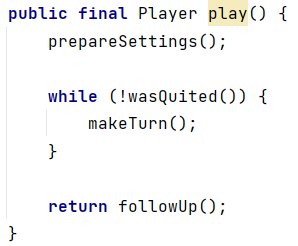
\includegraphics[width=8cm]{Bilder/templatePattern}}
\caption{Die Template-Methode play()}
\label{fig:templatePattern}
\end{figure}




\newpage
\section{Refactoring}
Refactoring wird dazu verwendet den Code durch Code Reviews übersichtlicher und/oder lesbarer zu machen. Dabei wird das Gesamtverhalten des bestehendem Codes nicht verändert. Nachdem Refactoring-Schritt sollte die Vorgehensweise des Programms immer noch die gleiche sein wie zuvor. Dabei können sich aber Fehler einschleichen, da möglicherweise etwas vergessen oder übersehen wurde.
Diese Stellen, die auf \glqq schlechten \grqq Code hinweisen, werden als Code Smells bezeichnet.



\subsection{Duplicated Code}
Wie der Name schon sagt, gibt es an mehreren Stellen Code, der für das Gleiche zuständig ist. Dies sollte vermieden werden, da zum einen der Code unnötig größer wird und, falls sich etwas an dieser Stelle ändern soll, muss das an zwei oder mehr Stellen getan werden. Um einen Gewinner nach einem Spielzug zu berechnen werden Spielregeln verwendet.

\begin{figure}[H]
\centering
{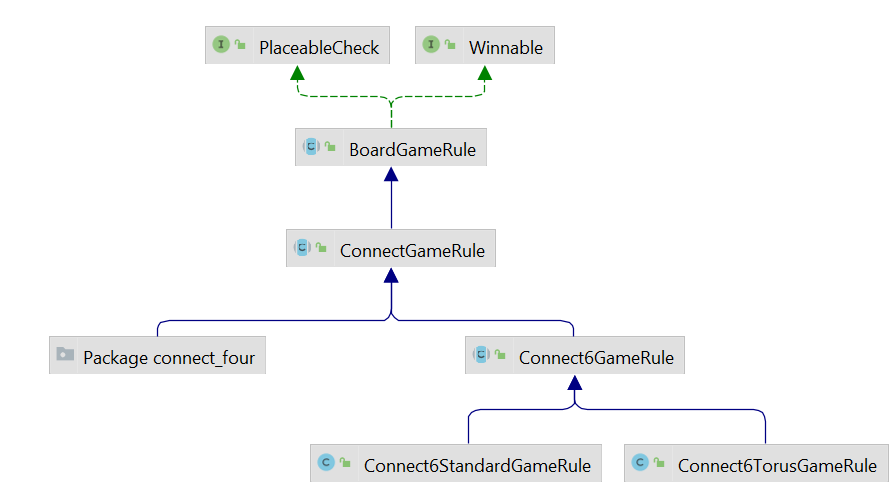
\includegraphics[height=4cm]{Bilder/ClassDiagGameRules}}
\caption{Klassendiagramm der Spielregeln}
\label{fig:ClassDiagGameRules}
\end{figure}

Ursprünglich wurden sowohl in der Connect6StandardGameRule und der Connect6-TorusGameRule berechnet ob ein Sieger vorliegt. Im Grundaufbau machen die beiden Klassen genau das Gleiche. Nur dass bei der Torus-Variante die Felder auch über den Rand hinaus gezählt werden. Zusätzlich wurde bei der Torus-Variante der Algorithmus auch sehr kompliziert programmiert. Aus diesen zwei verschiedene Implementierungen wurde dann eine in der Oberklasse Connect6GameRule. Somit kann diese Implementierung dann auch bei den Connect\_four Spielregeln verwendet werden. In ConnectGameRules wurde diese Methode dann wie bei der Connect6StandardGameRule programmiert und somit eine Method-Extraktion angewendet. Es wurde nur eine kleine Anpassung gemacht, sodass das nächste Feld, das betrachtet werden soll, in einer eigenen Methode bestimmt wird. Dies wird dann erst in den beiden Unterklassen definiert. Somit gibt es jetzt nur noch eine Implementierung die einen Gewinner berechnet.



\subsection{Shotgun Surgery \& Switch-Statement}
Dieses Problem tritt auf, wenn eigentlich nur eine Kleinigkeit angepasst werden soll aber dann tatsächlich an vielen Stellen Code angepasst werden muss. In meinem Fall kam noch hinzu, dass es sich um ein Enum gehandelt hat, dass auch in mehreren Switch-Statements verwendet wurde und die möglichen Befehle darstellen sollte. Wenn bisher aber ein neuer Befehl hinzukommen soll, musste an mindestens vier Stellen Code angepasst werden.
\\

\begin{figure}[htpb!]
\centering
\begin{subfigure}{.4\textwidth}
  \centering
  {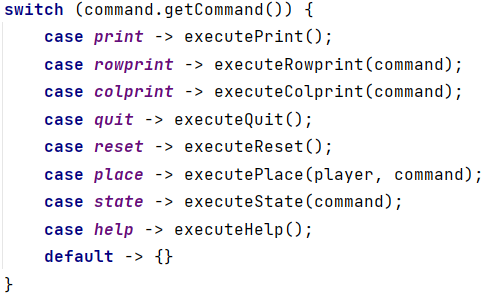
\includegraphics[height=4cm]{Bilder/Switch}}
  %\caption{A subfigure}
  \label{fig:sub1}
\end{subfigure}%
\begin{subfigure}{.6\textwidth}
  \centering
  {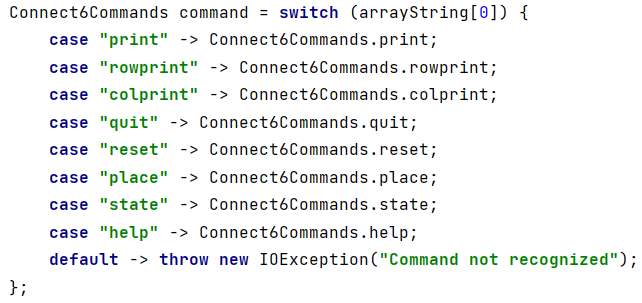
\includegraphics[height=4.2cm]{Bilder/Switch2}}
  %\caption{A subfigure}
  \label{fig:sub2}
\end{subfigure}
\caption{Mehrere Swtich-Statements für Befehle}
\label{fig:test}
\end{figure}

\noindent Jeder Befehl braucht folgende Informationen: 
\begin{itemize}
\item einen Text, der in der Konsole eingegeben werden muss um den Befehl zu adressieren
\item einen Enum, um den Befehl unabhängig der Eingabe zu machen z.B. case-insensitiv
\item eine Anzahl an korrekten Parametern
\item welche Methode angewendet werden soll
\end{itemize}

\noindent Daraus wurde dann eine neue Klasse gemacht, die alle diese Punkte in einem Objekt speichert. Zusätzlich dazu wurde noch eine Klasse erstellt, die auf Anfrage die richtigen Werte zurückgibt und die zuvor verwendeten Switch-Konstrukte ablöst. Damit wurde Replace Conditional with Polymorphism angewendet. Somit muss nur noch an zwei Stellen Änderungen gemacht werden. Zum Einen muss ein neues Enum definiert werden und zum Anderen müssen alle anderen Werte für diesen Befehl definiert werden. Damit sind die Befehle auch direkt im Spiel verwendbar werden.

\begin{figure}[H]
\centering
{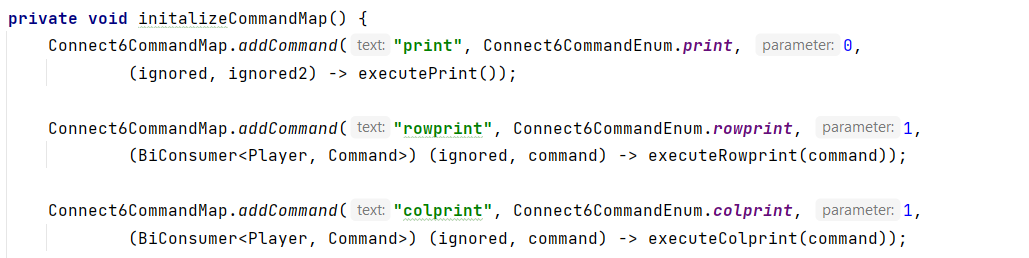
\includegraphics[height=4cm]{Bilder/CmdMap}}
\caption{Definition der Eigenschaften der Befehle}
\label{fig:CmdMap}
\end{figure}



\subsection{Long Method}
Dieses Problem taucht an mehreren Stellen im Code auf. Zwar gibt es so gut wie keine Methode, die länger als 20 Zeilen ist aber bei manchen Methoden ist selbst das zu viel und sorgt für Probleme beim Lesen der Klasse. Je nach Person ist die akzeptable Länge auch unterschiedlich. Bei mir sind das ungefähr 10 Zeilen pro Methode. Dies halte ich auch an vielen Stellen ein aber an vielen Stellen eben auch nicht, wie in der Connect6-Klasse.

\begin{figure}[H]
\centering
{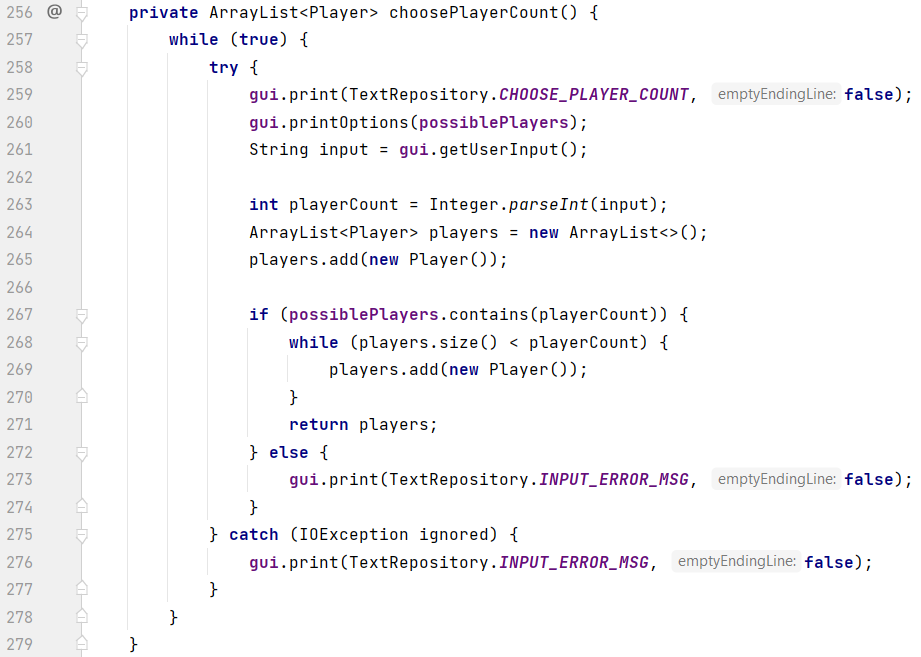
\includegraphics[width=15cm]{Bilder/longMethod}}
\caption{Beispiel für lange Methoden}
\label{fig:CmdMap}
\end{figure}




\end{document}